% Please use the skeleton file you have received in the
% invitation-to-submit email, where your data are already
% filled in. Otherwise please make sure you insert your
% data according to the instructions in PoSauthmanual.pdf
\documentclass{PoS}
\usepackage[utf8x]{inputenc}
\usepackage{wrapfig}\usepackage{wrapfig} % Allows wrapping text around tables and figures
\usepackage{graphicx}
\usepackage{subcaption}
\usepackage{float}
\newcommand{\bbbar}{$b\bar{b}$}
\newcommand{\afb}{$A_{FB}^b$}
\newcommand{\sm}{Standard Model}
\newcommand{\bsm}{Beyond Standard Model}
\newcommand{\mF}{\mathcal{F}^I} % Allows wrapping text around tables and figures

%\usepackage{wrapfig}

\usepackage{lineno}
\usepackage{array}
\usepackage{lscape}
\usepackage{graphicx}
\usepackage{subcaption}
\usepackage{float}
\usepackage{multicol} % This is so we can have multiple columns of text side-by-side
\usepackage{amsmath}
\columnsep=100pt % This is the amount of white space between the columns in the poster
\columnseprule=3pt % This is the thickness of the black line between the columns in the poster

\usepackage[svgnames]{xcolor} % Specify colors by their 'svgnames', for a full list of all colors available see here: http://www.latextemplates.com/svgnames-colors

\usepackage{times} % Use the times font
%\usepackage{palatino} % Uncomment to use the Palatino font

\usepackage{graphicx} % Required for including images
\graphicspath{{figures/}} % Location of the graphics files
\usepackage{booktabs} % Top and bottom rules for table
\usepackage[font=small,labelfont=bf]{caption} % Required for specifying captions to tables and figures
\usepackage{amsfonts, amsmath, amsthm, amssymb} % For math fonts, symbols and environments
\usepackage{wrapfig} % Allows wrapping text around tables and figures

\newcommand{\bbbar}{$b\bar{b}$}
\newcommand{\afb}{$A_{FB}^b$}
\newcommand{\sm}{Standard Model}
\newcommand{\bsm}{Beyond Standard Model}
\newcommand{\mF}{\mathcal{F}^I}

\title{Studies of $ e^+e^-\to b\bar{b}$ channel at the International Linear Collider}

\ShortTitle{Studies of $ e^+e^-\to b\bar{b}$ channel at the International Linear Collider}

\author{\speaker{Sviatoslav BILOKIN}\\%thanks{A footnote may follow.}\\
        Laboratoire de l'Acceler\'ateur Lin\'eare\\
        E-mail: \email{bilokin@lal.in2p3.fr}}

\author{Roman P\"OSCHL\\
        Laboratoire de l'Acceler\'ateur Lin\'eare\\
        E-mail: \email{poeschl@lal.in2p3.fr}}

\author{Fran\c cois RICHARD\\
	Laboratoire de l'Acceler\'ateur Lin\'eare\\
	E-mail: \email{richard@lal.in2p3.fr\\
		\\}
	\hspace{20pt}on behalf of the ILD concept group}

\abstract{
	The top and bottom quarks plays a central role in the quest for new physics. The complementarity between studies of electroweak top quark production and bottom quark production is therefore intuitively clear and pointed out in the literature.
	The tension between the LEP measurement and the Standard Model prediction of the forward-backward asymmetry \afb\ is still one of the unsolved questions in the field and may be interpreted as a first manifestation of New Physics in the heavy quark sector. The process $e^+e^-\to b\bar{b}$ at the ILC offers a unique opportunity for a final word on the tension. Polarised beams allow for a large disentangling of the coupling constants or form factors that govern the $Z^0/\gamma b \bar{b}$ vertex.
	
	%These studies are based on a detailed simulation study of the process $e^+e^-\to b\bar{b}$ at 250\,GeV with the ILD Detector. Besides the phenomenological implications, the studies demonstrate that with a careful analysis of the final state the charge of the b-quarks can be determined on an event-by-event basis with the ILD Detector. Such a capability is unprecedented by past and present particle physics experiments.
	}

\FullConference{EPS-HEP 2017, European Physical Society conference on High Energy Physics\\
		5-12 July 2017\\
		Venice, Italy}

\begin{document}

\section{Introduction}
The LEP~I collaborations have determined the $b$-quark couplings to the $Z^0$ boson by measuring the $b$ partial width and the forward-backward asymmetry called \afb. These quantities provide the most precise value of $\sin^2\theta_W$ at LEP~I. It turns out that this value is about three standard deviations~\cite{Baak:2014ora} away from the very precise value from SLD using beam polarisation, see Fig.~\ref{fig:ewfit}. Redoing precisely this measurement is therefore a priority for future $e^+e^-$ colliders. 


\begin{figure}
	{\centering
		%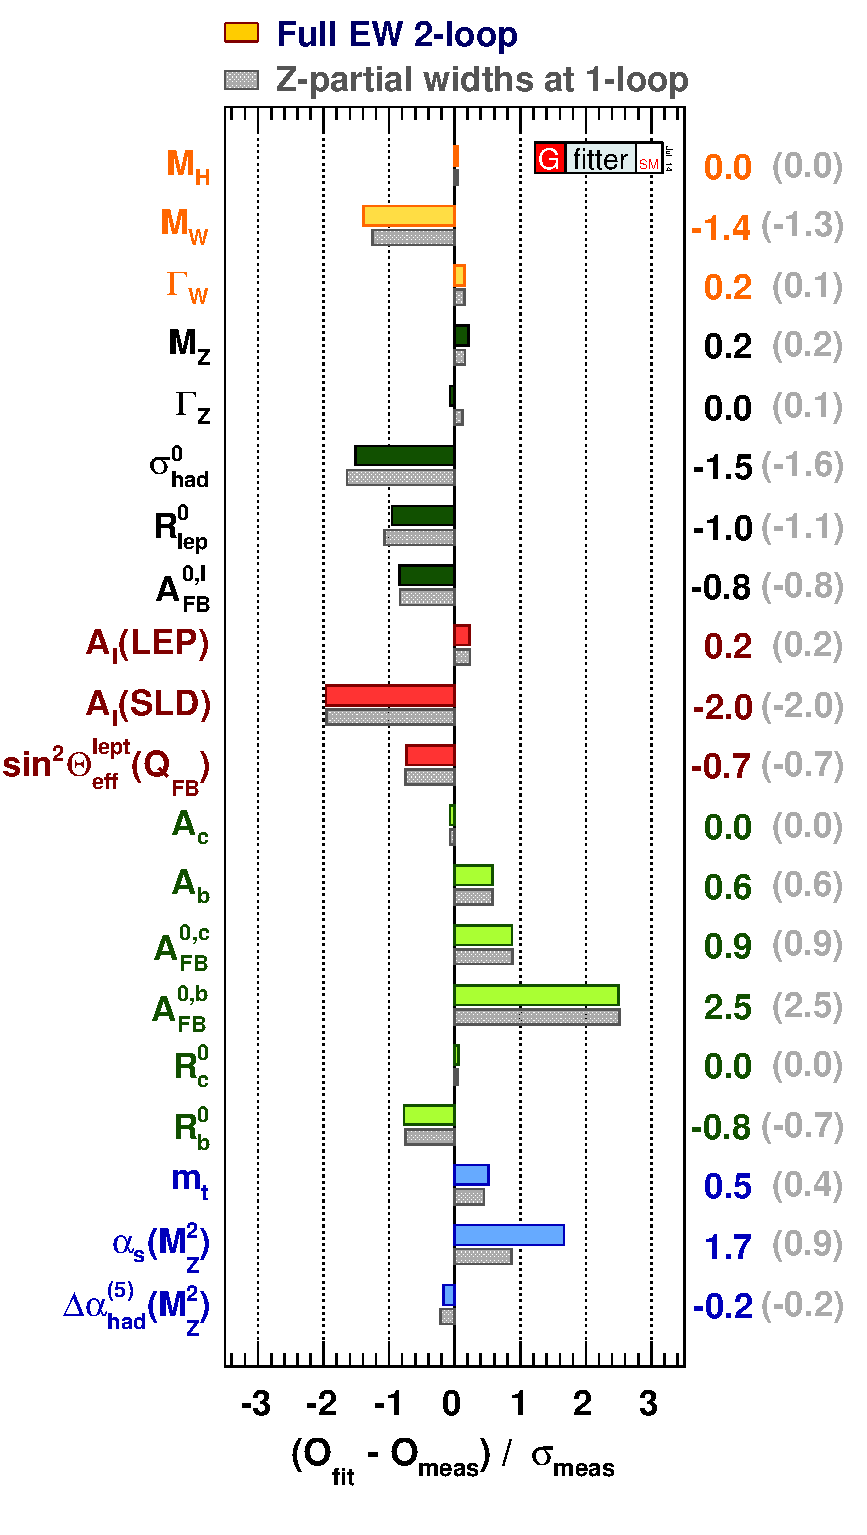
\includegraphics[width=0.55\linewidth]{../graphics/2014_07_16_PullPlotTwoBarsTwoTheos_logo-eps-converted-to.pdf}
		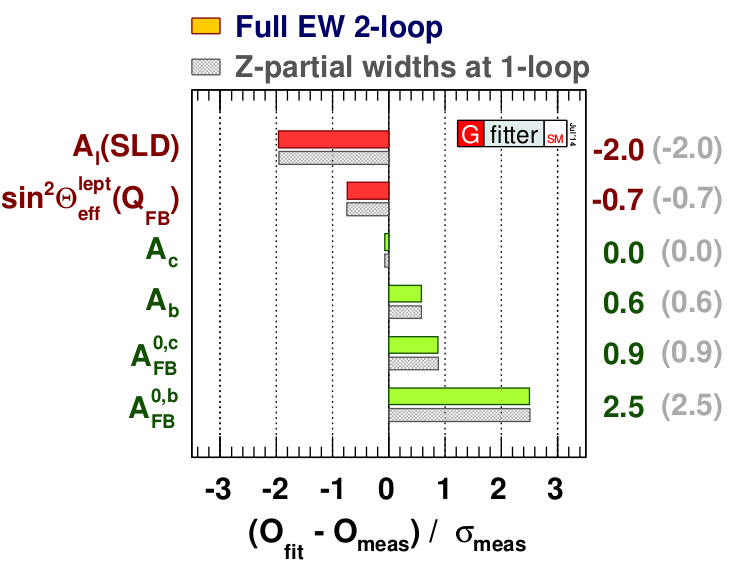
\includegraphics[width=0.45\linewidth]{../poster/figures/deviation2.png}
		\caption{\sl Deviations of the electroweak precision
			observables in the Standard Model. Extracted from~\cite{Baak:2014ora}. }
		\label{fig:ewfit}
	}
\end{figure}

In this study, we intend to prove that the International Linear Collider (ILC)~\cite{Behnke:2013xla}, with {polarised beams and high luminosity}, offers a unique opportunity for precise measurements well above the resonance, where both $Z^0$ and photon exchanges are present. 
This additional complexity turns out to be of a great advantage since it allows, through $\gamma - Z^0$ interference, to be sensitive to the sign of $Z^0$ couplings and fully solve the LEP~I puzzle in an unambiguous way. 
More details are given in~\cite{Bilokin:2017lco}.
Recall that the LEP~I anomaly can be interpreted up to a sign ambiguity for what concerns the right-handed coupling $Z^0 b\bar{b}$, referred hereafter as $g_R^Z$, which shows the largest deviation~\cite{Djouadi:2006rk}.

\begin{figure}
	{\centering
		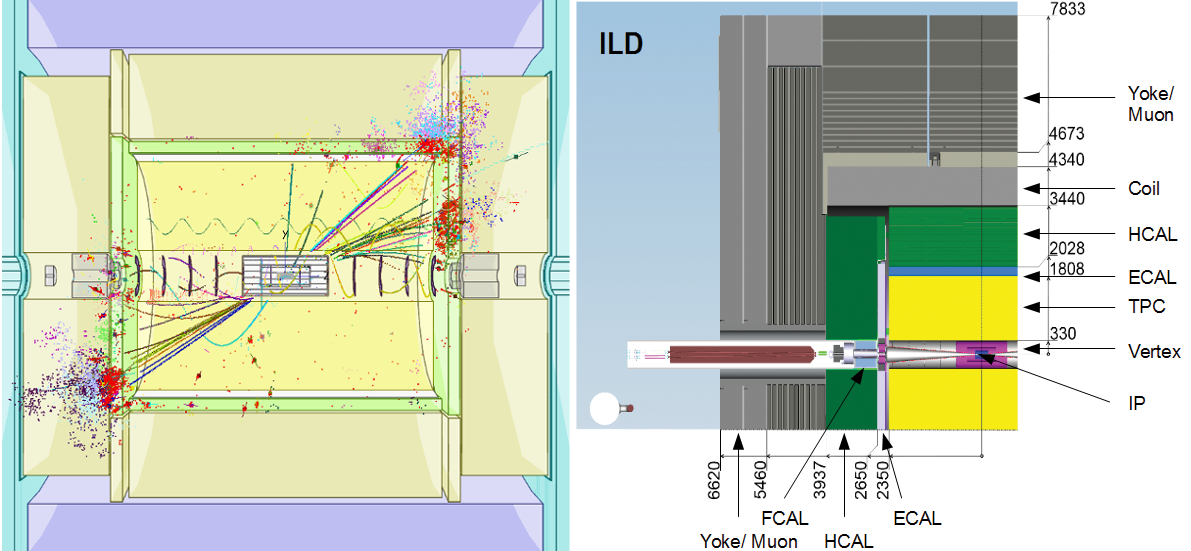
\includegraphics[width=0.8\linewidth]{../poster/figures/ild3.png}
		\caption{\sl Example of the event display of the $e^+ e^-\to b\bar{b}$ process in a full simulation of the ILD detector (left) and schematic view of the ILD concept~\cite{Behnke:2013lya} (right). }
		\label{fig:ILDScheme}
	}
\end{figure}

%The schematic view of the ILC accelerator complex is shown in Fig.~\ref{fig:ILCScheme}.
In this work, the $e^+ e^-\to b\bar{b}$ channel is studied at $\sqrt{s}=250$\,GeV using full simulation of the ILD experiment~\cite{Behnke:2013lya}, which include beam spectrum and initial state radiation modelling.
The high-granularity of the ILD subdetectors allows for an individual particle reconstruction using the Particle Flow approach~\cite{Marshall:2015rfa}.
The schematic view of the ILD concept and the subdetector layout is presented in Fig.~\ref{fig:ILDScheme}.



\section{$b$-quark charge sign assignment}

The $b$-quark polar angle reconstruction requires an accurate $b$-quark charge sign assignment. 
The $b$-quark charge is identified using two basic signatures:
\begin{itemize}
	\item \textbf{Vertex charge} is a sum of all reconstructed charges, which are associated to the $B$-hadron vertices;
	\item \textbf{Kaon charge} is a charge of charged kaons found in $b$-hadron vertices. 
\end{itemize}

Figure ~\ref{fig:vtx} shows a schematic view of a b-hadron decay-chain as seen in the ILD vertex detector.
%The schematic appearance of $b$-hadron decays in the ILD Vertex Detector is presented in Fig.~\ref{fig:vtx}.

\begin{figure}
	{\centering
		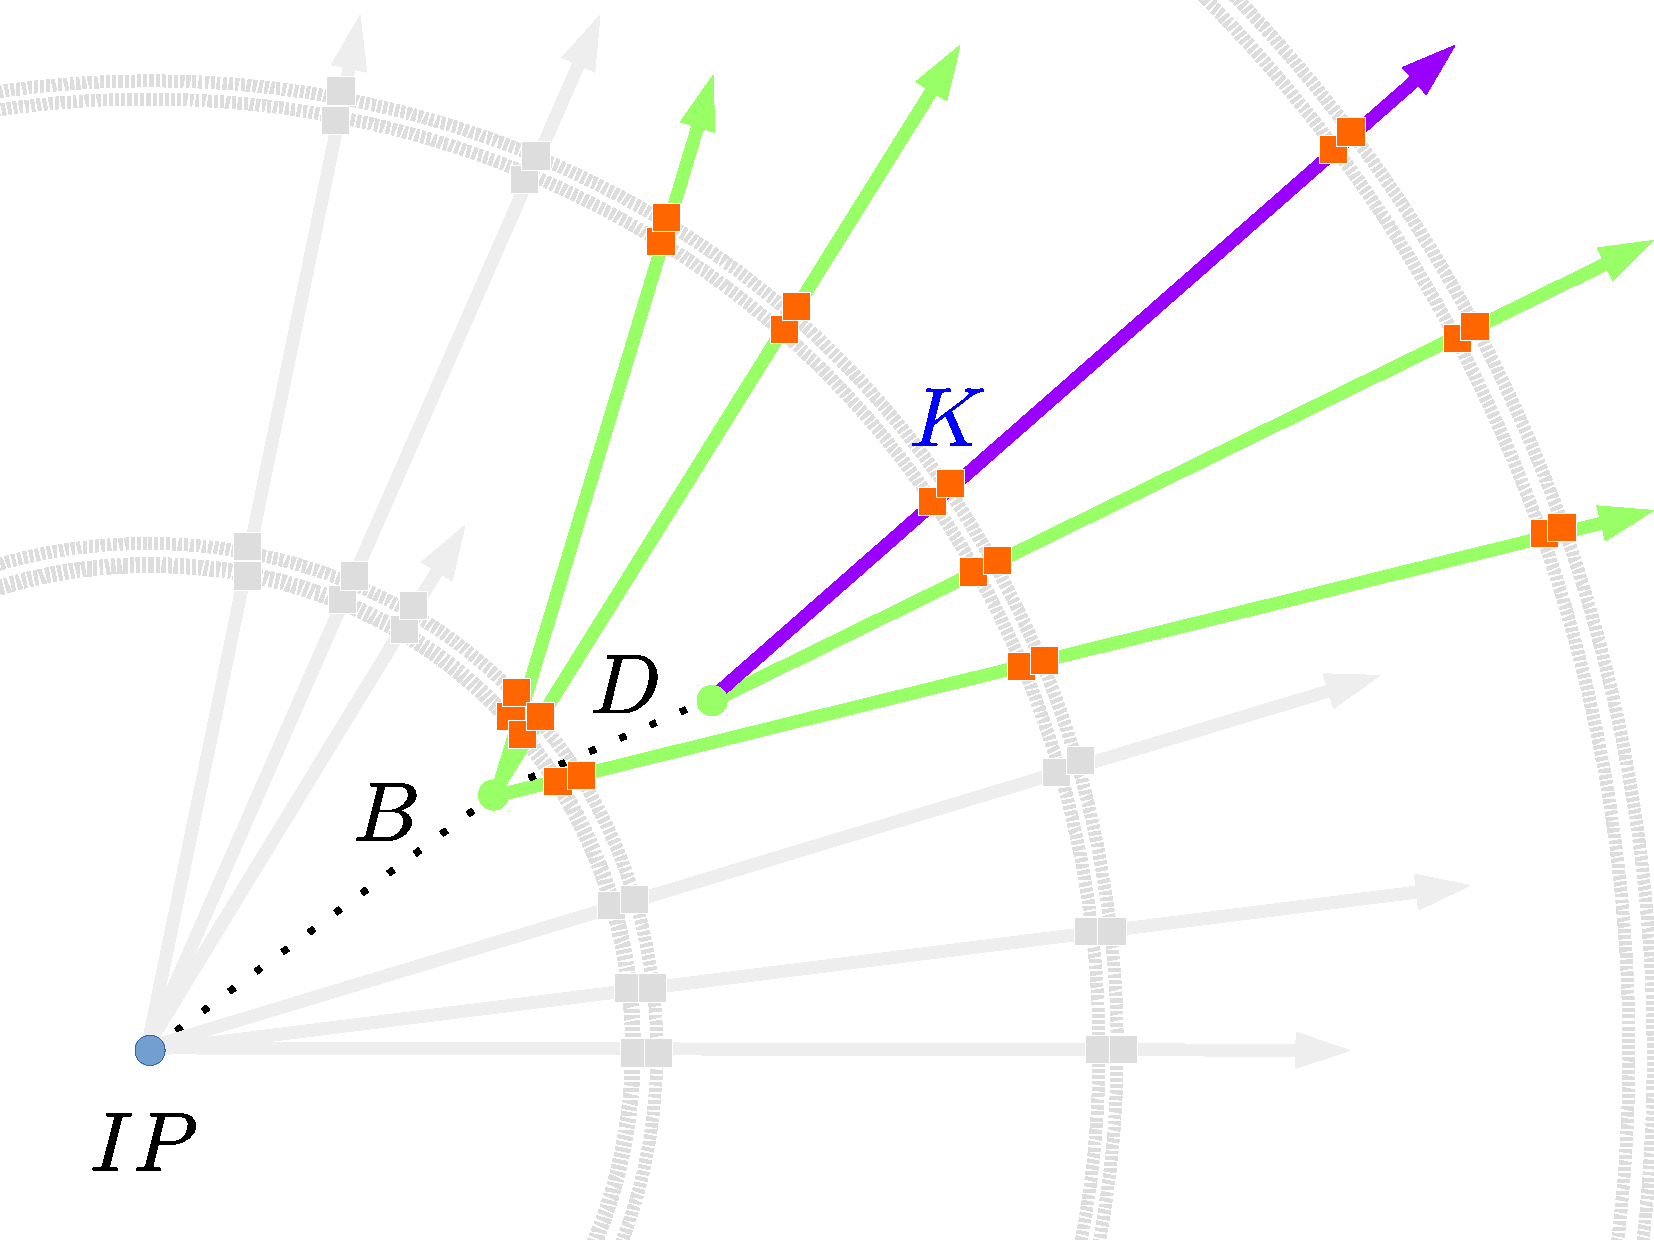
\includegraphics[width=0.4\linewidth]{../poster/figures/vtx.pdf}
		\caption{\sl Illustration of $b$-hadron decays. }
		\label{fig:vtx}
	}
\end{figure}
It was found that vertexing algorithms can miss one or more $b$-hadron decay particles from the reconstructed vertices, which decreases the purity of the reconstructed vertex charges.
A vertex recovery procedure has been developed to identify the missed tracks and to add them back to the vertices. Figure~\ref{fig:thetaepsilonsys} shows that this improves the vertex charge reconstruction considerably.
%The developed Vertex Charge Recovery procedure enhances the vertex charge purity by adding the missing $b$-hadron particles back to the measured vertices using a set of reconstructed observables. 


%The kaon identification is possible using the TPC $dE/dx$ information. 
The charged kaons are identified using the specific energy-loss
$dE/dx$ in the TPC.
After correcting for the angular dependence of $dE/dx$, the charged kaons from $b$-hadron vertices can be identified with 97\% purity and 87\% efficiency, assuming 5\% precision on the energy loss value.
The plots of the $dE/dx$ as function of particle momentum for different hadrons are shown in Fig.~\ref{fig:lepsilonsys}.

	\begin{figure}
		\centering
		\begin{subfigure}{0.5\textwidth}
			\centering
			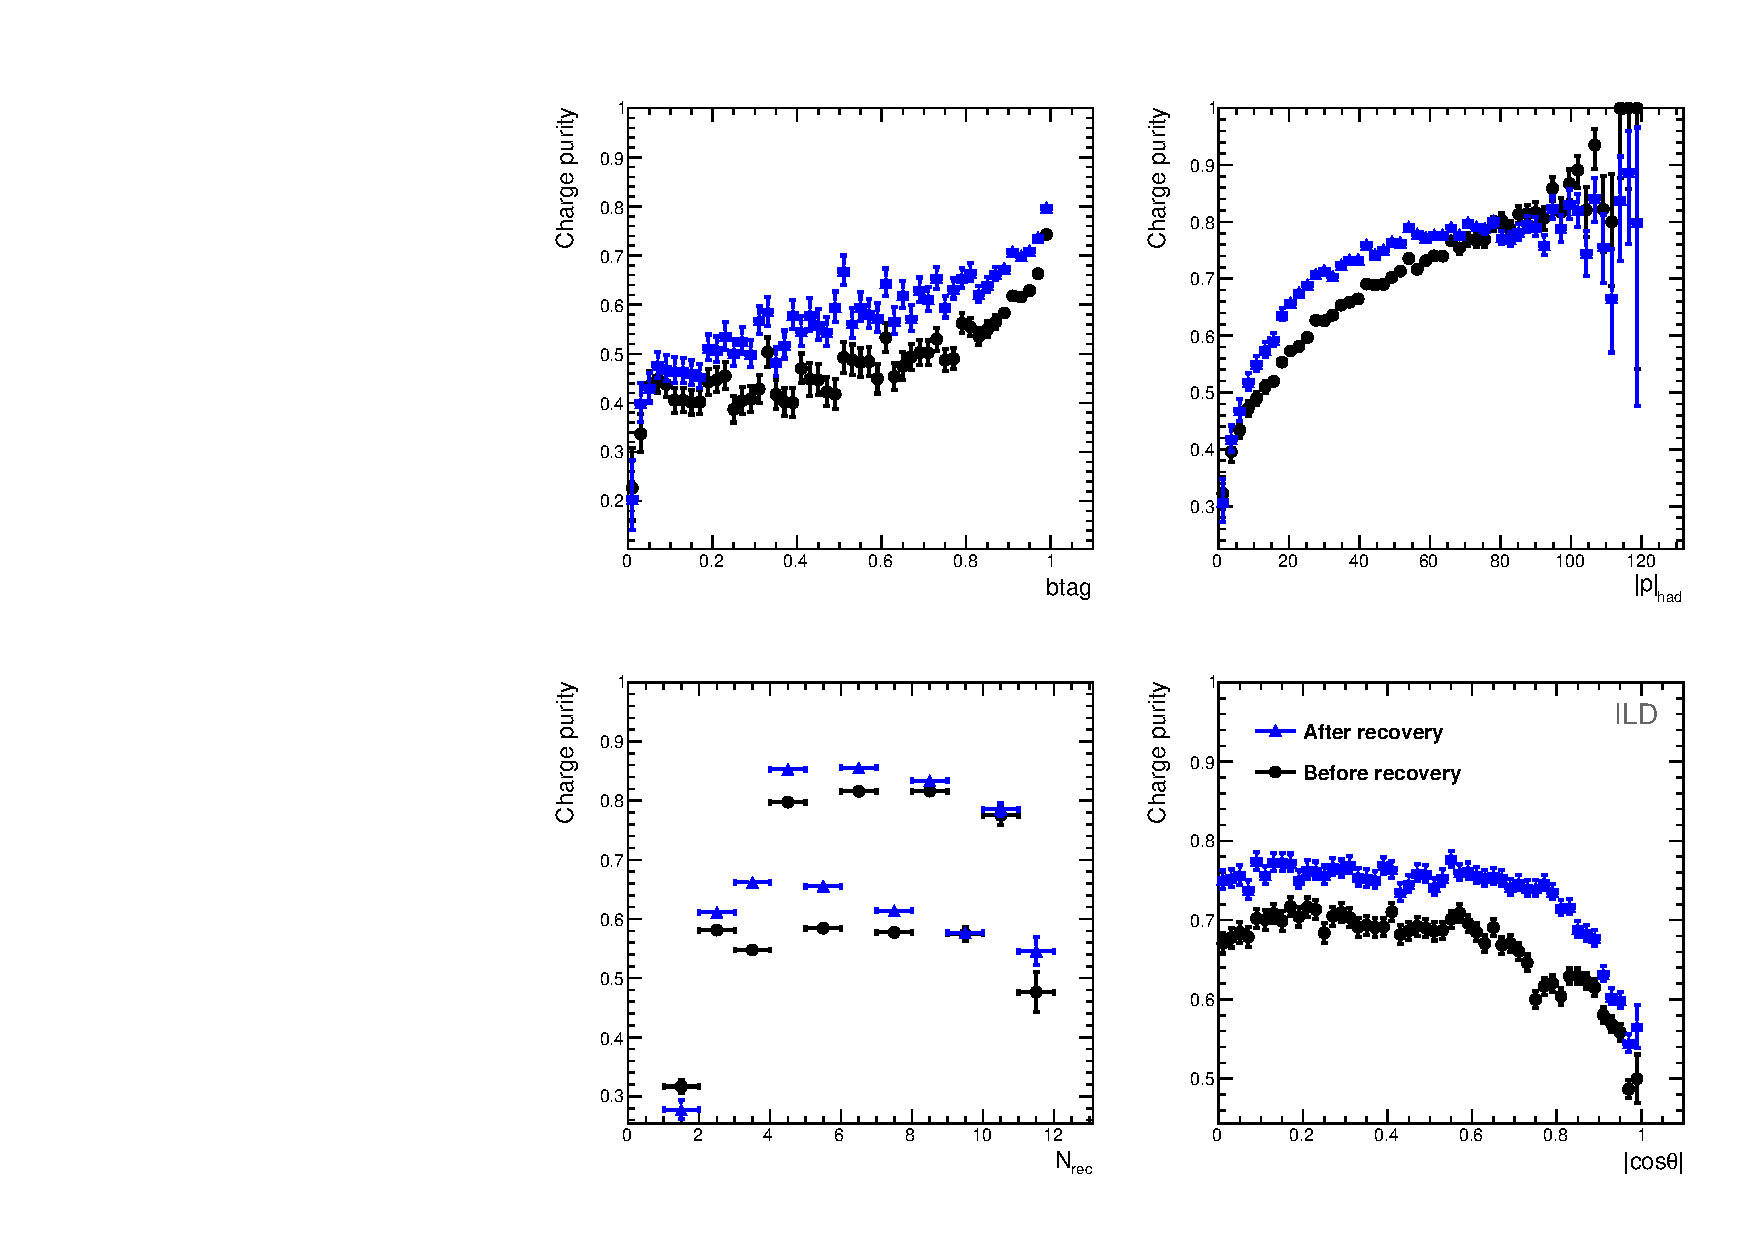
\includegraphics[clip, trim=10cm 0cm 0cm 10cm,width=0.95\linewidth]{../poster/plots/purity-recovery-ild.pdf}
			\caption{\label{fig:thetaepsilonsys} }
		\end{subfigure}% 
		\begin{subfigure}{0.5\textwidth}
			\centering
			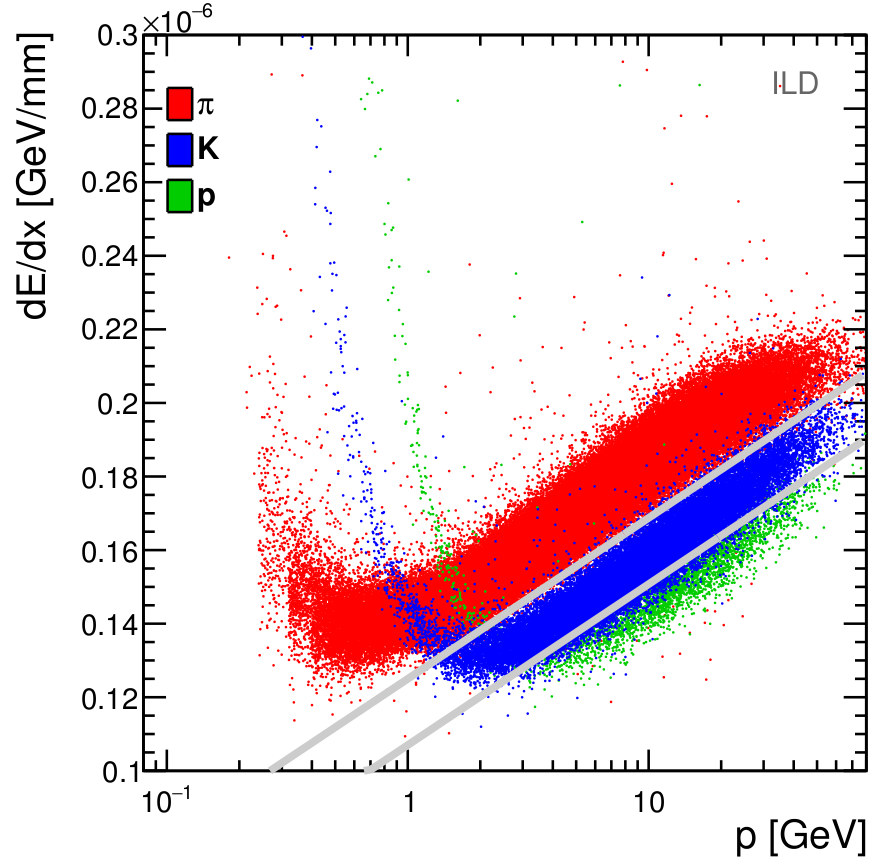
\includegraphics[width=0.87\linewidth]{../poster/plots/dedx2.png}
			\caption{\label{fig:lepsilonsys} }
		\end{subfigure}
		\caption{\label{fig:Charges_3} \sl Vertex charge sign assignment purity as function of $|\cos\theta|$ (left) and energy deposition per unit of length $dE/dx$ as function of particle momentum $p$ (right).}
	\end{figure}
	
\section{$b$-quark polar angle spectrum}

The reconstructed $b$-quark polar angle distributions at $\sqrt{s} = 250$\,GeV using a combination of kaon and vertex charge signatures are shown in Fig.~\ref{fig:BAsymmetryFinal_3}. The integrated luminosity $\mathcal{L}_I = 250$\,fb$^{-1}$ is assumed for each beam polarisation.


\begin{figure}
	\centering
	\begin{subfigure}{0.5\textwidth}
		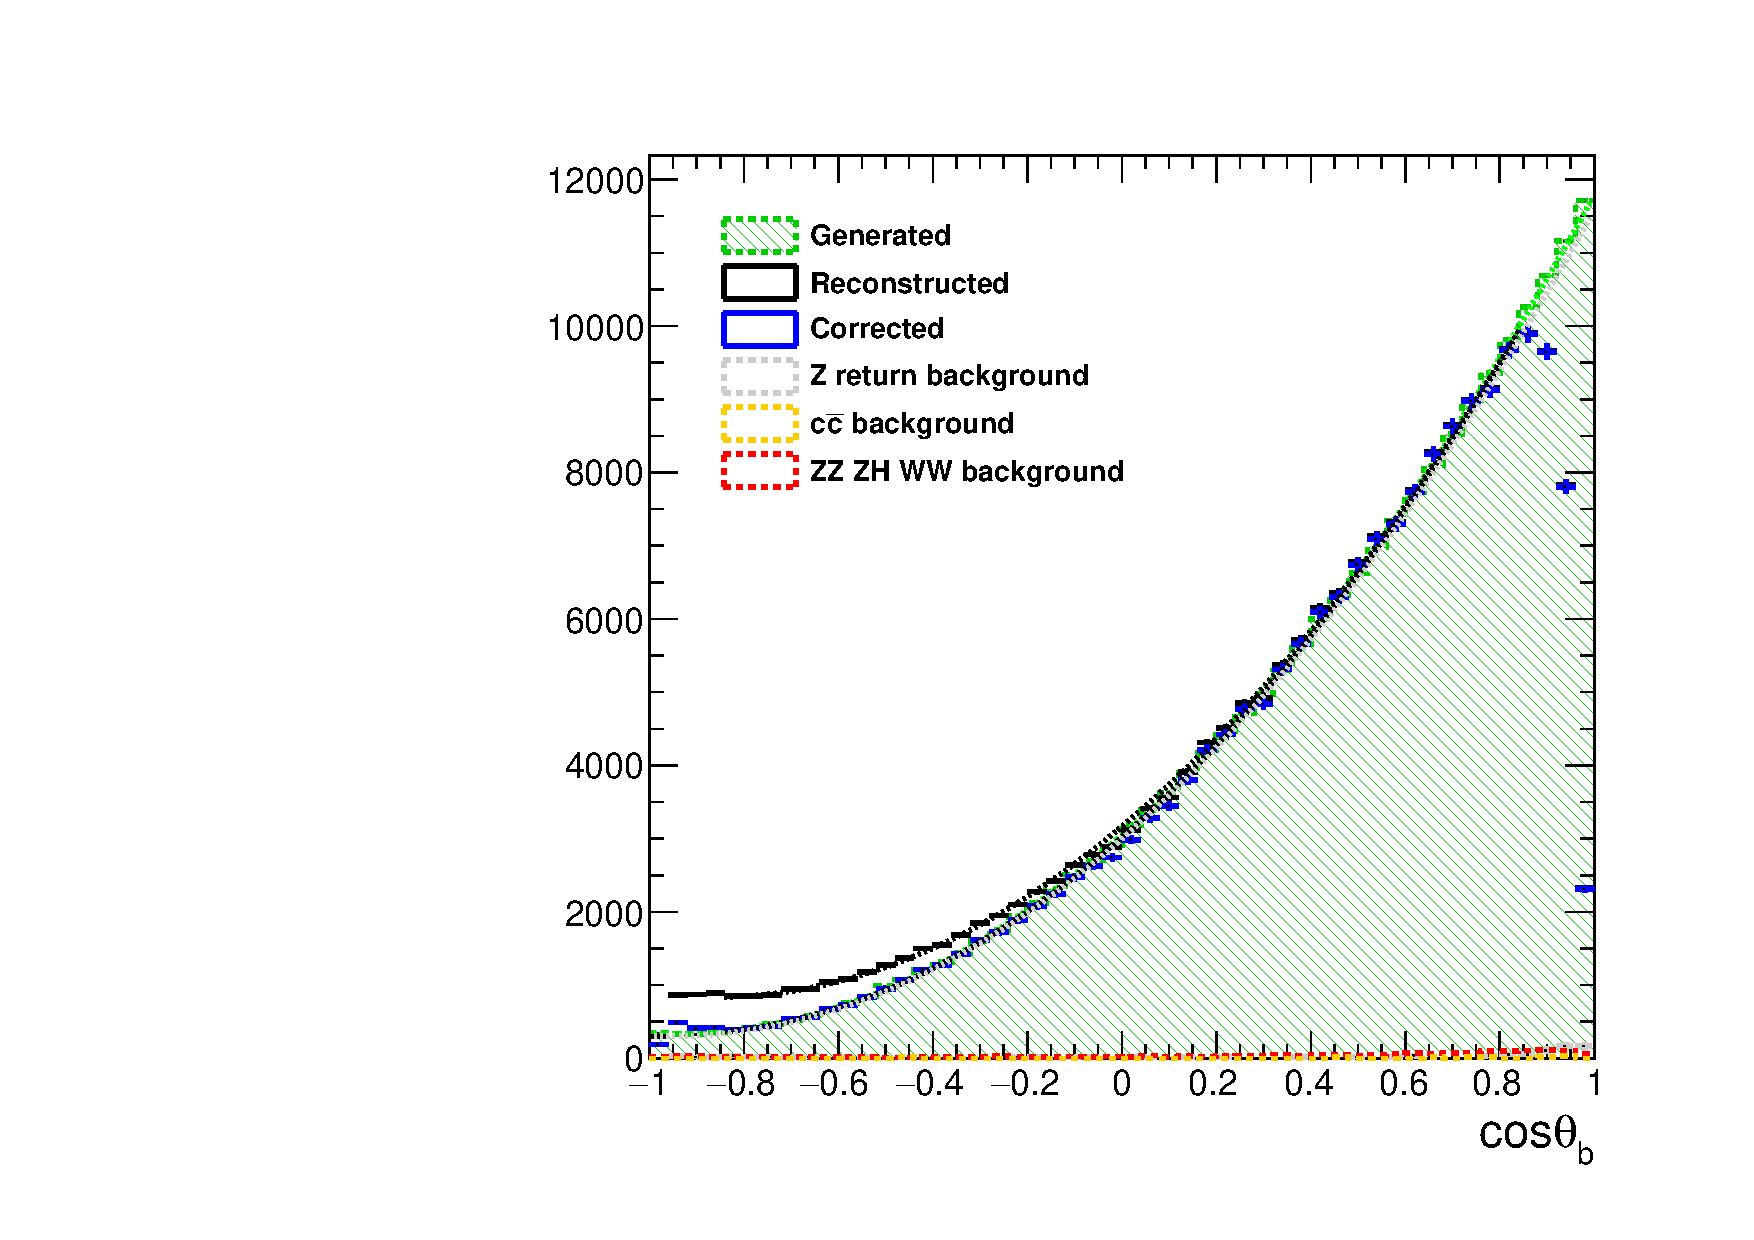
\includegraphics[width=0.95\textwidth]{../ILD/plots/basymmetry-final-left.pdf}
		\llap{\shortstack{%
				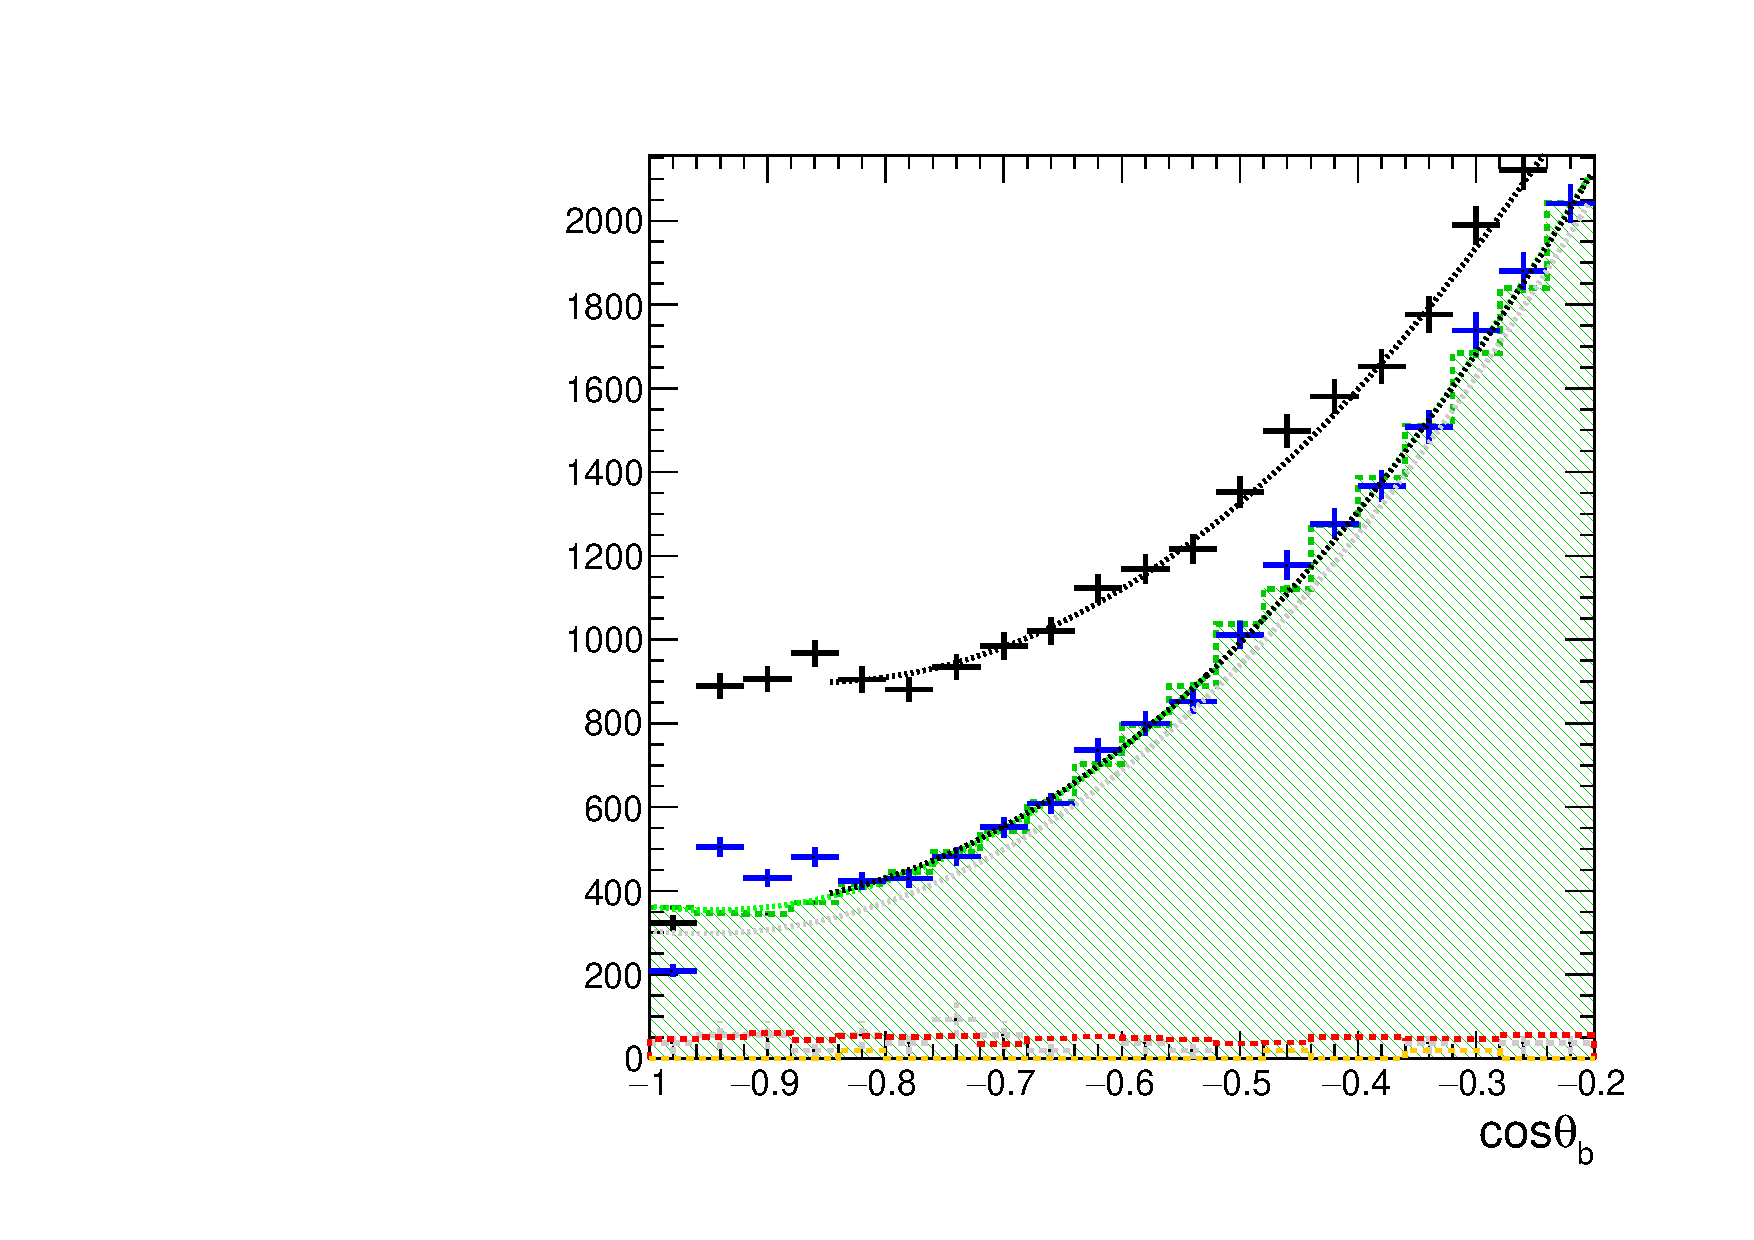
\includegraphics[clip, trim=0cm 0cm 1.8cm 1.7cm, scale=.14]{../ILD/plots/zoom-final.pdf}\\
				\rule{0ex}{0.51in}%
			}
			\rule{1.8in}{0ex}}
		\caption{\label{fig:BAsymmetryFinal_a_3} }
	\end{subfigure}% 
	\begin{subfigure}{0.5\textwidth}
		\centering
		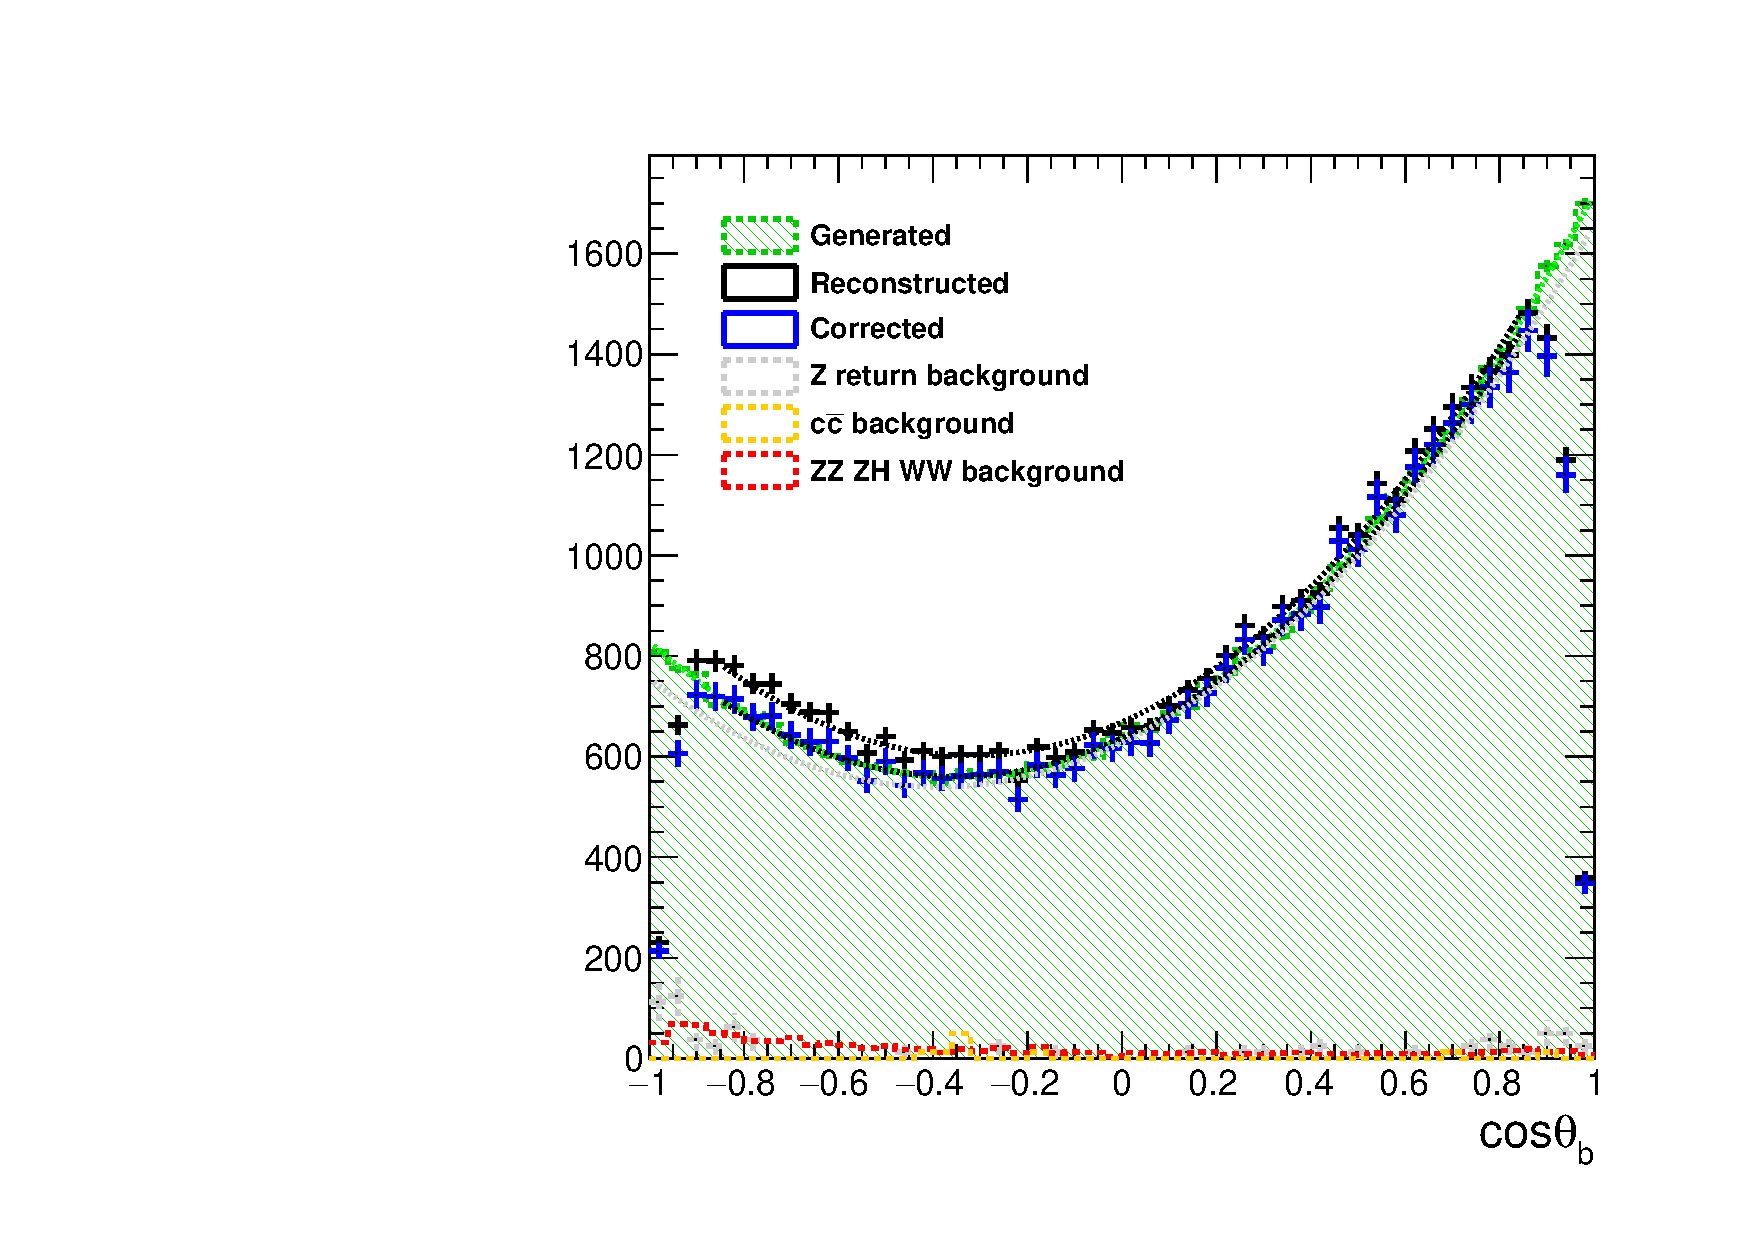
\includegraphics[width=0.95\textwidth]{../ILD/plots/basymmetry-final-right.pdf}
		\caption{\label{fig:BAsymmetryFinal_b_3} }
	\end{subfigure}
	\caption{\sl Generated $b$-quark polar angle distribution compared to the final reconstructed $b$-quarks polar angle in left-handed case (a) and right-handed case (b) with overlaid background processes.  }
	\label{fig:BAsymmetryFinal_3}
\end{figure}

%The kaon and vertex charge purity is defined using the measured events with misreconstructed charges. 
The events with reconstructed kaon or vertex charges, which are incompatible between jets, allow to define the kaon and vertex charge purity in-situ.
Using the in-situ purities, the reconstructed spectrum is corrected using a data-driven procedure.
The corrected distributions are fitted by a general cross section function, defined as ${	S (1+\cos^2\theta) + A \cos\theta}$. The extracted precision on the $S$ and $A$ parameters is rescaled to the expected polarisation $e^-_L, e^+_R = \pm0.8, \mp0.3$ and to the luminosity sharing of the ILC physics program.
As one can see from Fig.~\ref{fig:BAsymmetryFinal_3}, the contribution of the diboson background processes is small. 

\section{Interpretation}

The relative precisions on the $Z^0b\bar{b}$ couplings, $g_L^Z$ and $g_R^Z$, for the LEP~I measurements and for the expected ILC performance are shown in Fig.~\ref{fig:LEPILCResult_3}. 
The ILC precision on the $g_R^Z$ coupling is enough to fully confirm or discard any New Physics influence on the $b$-quark electroweak couplings. 


\begin{figure}
	\centering
	\begin{subfigure}{0.5\textwidth}
		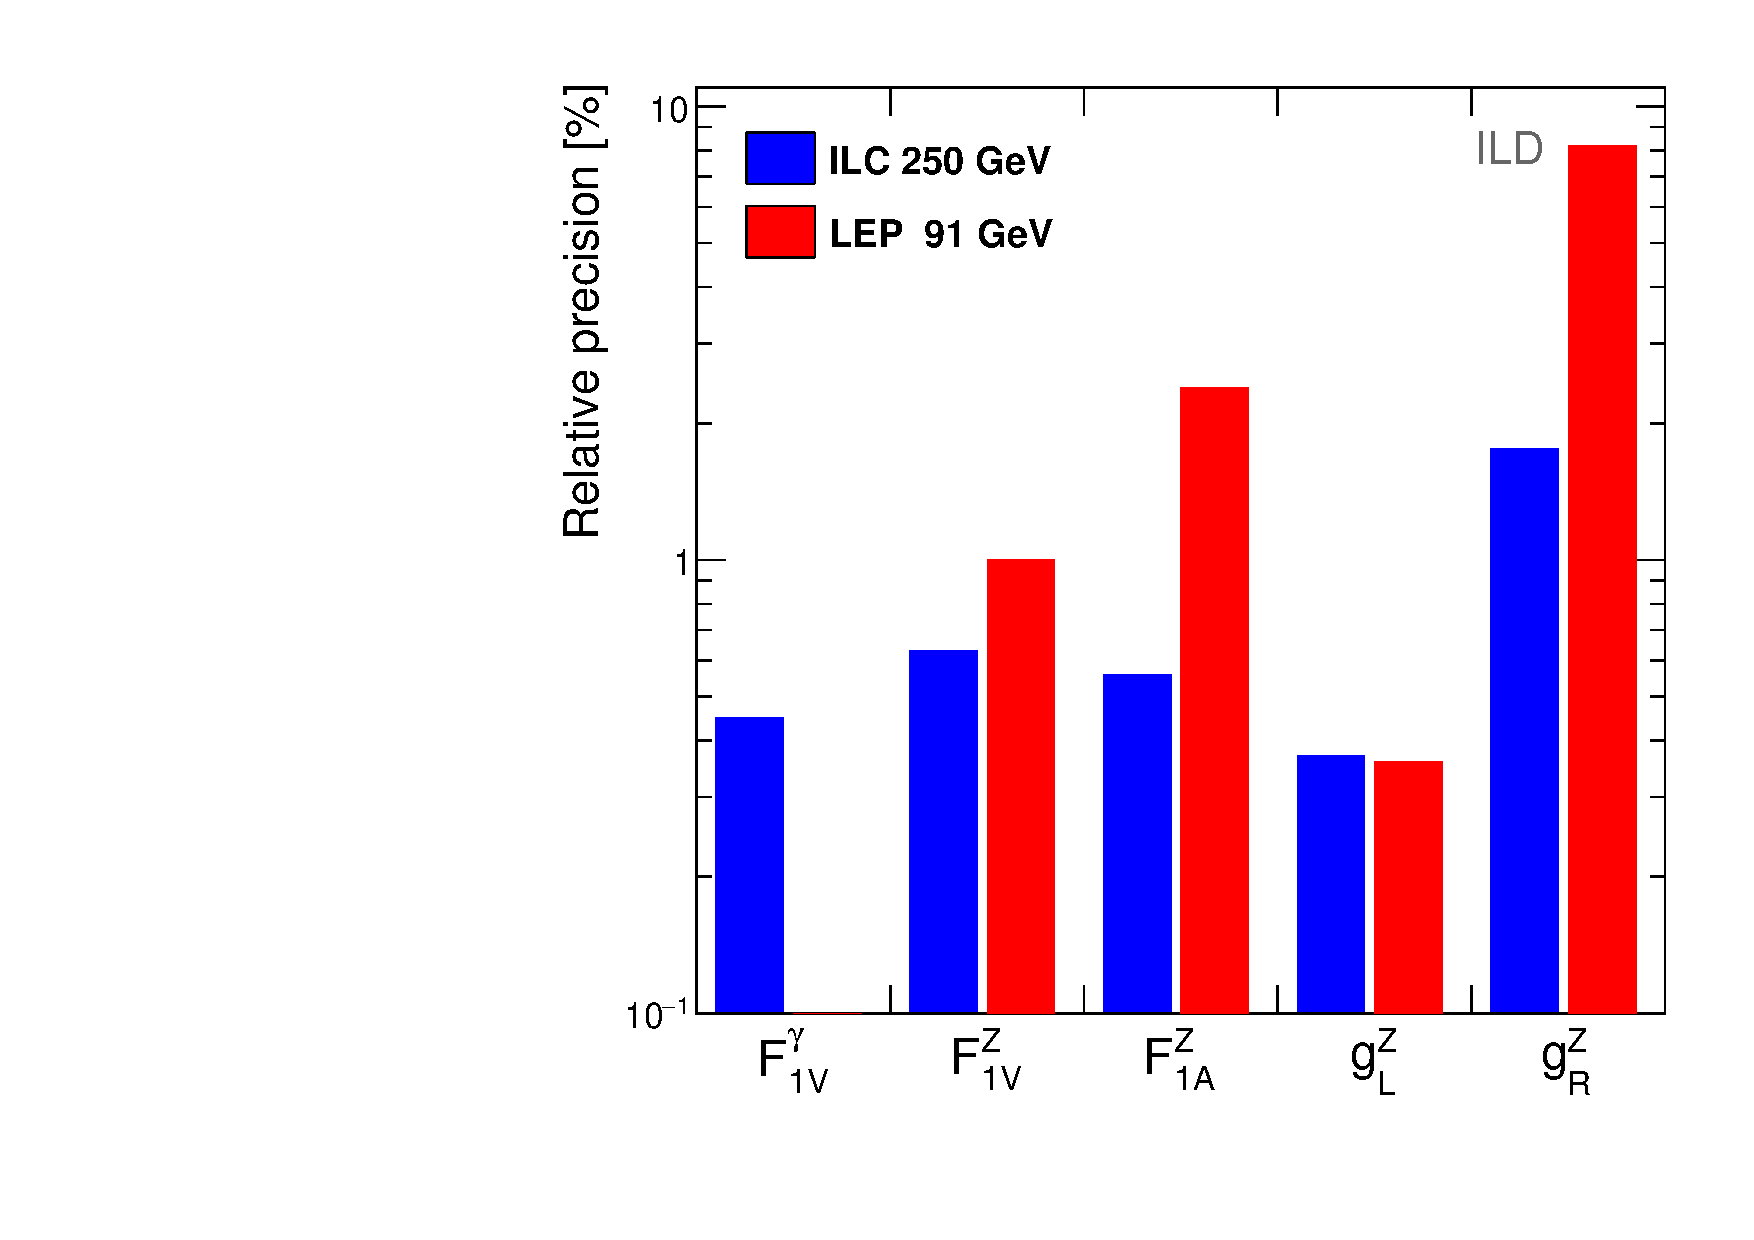
\includegraphics[width=0.95\linewidth]{../poster/plots/final-graph-ild.pdf}
		\caption{\label{fig:LEPILCResult_3_a} }
	\end{subfigure}% 
	\begin{subfigure}{0.5\textwidth}
		\centering
		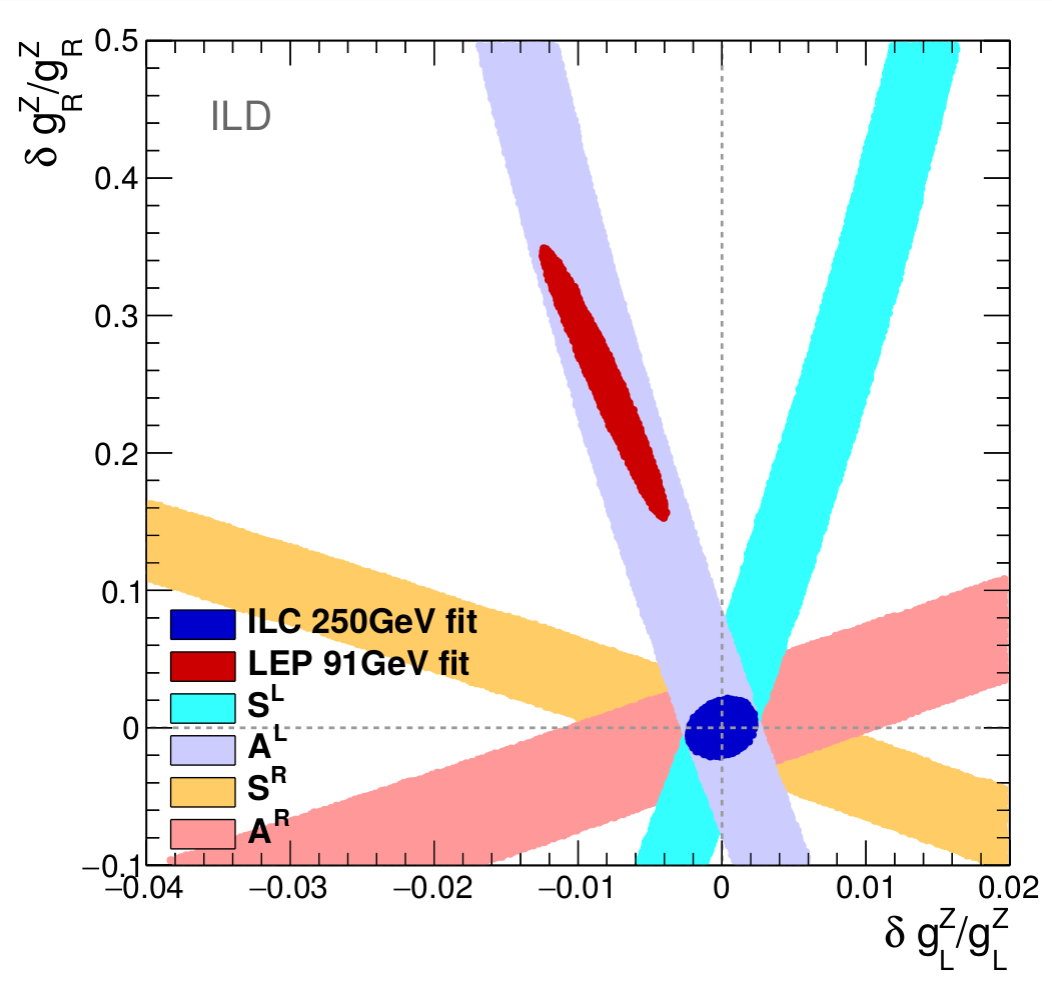
\includegraphics[width=0.95\linewidth]{../poster/plots/ilc-precision-ild.png}
		\caption{\label{fig:LEPILCResult_3_b} }
	\end{subfigure}
	\caption{\sl  Comparison of the LEP measurements to the expected precision at the ILC. The results of the ILC assume an integrated luminosity of $\mathcal{L_I} = 500$\,fb$^{-1}$ shared between beam polarizations at $\sqrt{s} = 250$\,GeV. }
	\label{fig:LEPILCResult_3}
\end{figure}

%--------------------------------------------------------------------------------
%	CONCLUSIONS
%--------------------------------------------------------------------------------

\section*{Conclusions}

\begin{itemize}
	\item The developed procedure of the $b$-quark charge reconstruction allows for measuring the $b$-quark polar angle. The residual impurity is corrected by a data-driven procedure;
	\item The $b$-quark polar angle fit allows for an independent determination of four electroweak couplings of the $b$-quark. The fit can be extended to also include a term proportional to $\sin^2\theta$, giving access to an independent determination of the tensorial couplings;
	\item  The relative precision on the right-handed coupling $dg^Z_R/g^Z_R\approx 2$\% at the ILC is sufficient to confirm at $>5\,\sigma$ or to discard the LEP~I effect, which is at the 25\% level.
	%\item A reach of new particle mass scale $\Lambda \approx 10$\,TeV is achievable for indirect New Physics searches using Effective Field theory approach.
	%\item The statistical precision after the first $\sqrt{s} = 250\,$GeV ILC program will be almost 5 times better than at LEP;
\end{itemize}


\section*{Forthcoming Research}
The $b$-quark charge technique can be applied to the fully hadronic $t\bar{t}$ decays and combine the results with semileptonic $t\bar{t}$ channel.
The kaon charge method can be extended on the $c$-quark polar angle analysis, where one can improve on the LEP~I results on the c-quark couplings precision. 
%Hence, at the ILC one can measure the top, bottom and charm quark electroweak couplings with an excellent sensitivity to New Physics effects.

\section*{Acknowledgements}
We would like to thank our collegues in the ILD group, in particular the software group, which developed the the simulation framework and produced the data samples used in this study.
%These studies are done using the full ILD simulation and we acknowledge the work of the ILD software and simulation groups.



%%%%%%%%%%%%%%%%%%%%%%%%%%%%%%%%%%%%%%%%%%%%%%%%%%%%%%%%%%%%%%%%%%%%%%%%%%%%%%%
%\bibliographystyle{unsrt} % Plain referencing style
%\bibliography{../mainbib} 

%\bibliography{../../OLD/Paper/mainbib}

\begin{thebibliography}{99}
%\cite{Baak:2014ora}
\bibitem{Baak:2014ora} 
M.~Baak {\it et al.} [Gfitter Group],
%``The global electroweak fit at NNLO and prospects for the LHC and ILC,''
Eur.\ Phys.\ J.\ C {\bf 74}, 3046 (2014)
doi:10.1140/epjc/s10052-014-3046-5
[arXiv:1407.3792 [hep-ph]].
%%CITATION = doi:10.1140/epjc/s10052-014-3046-5;%%
%344 citations counted in INSPIRE as of 08 Oct 2017


%\cite{Behnke:2013xla}
\bibitem{Behnke:2013xla} 
T.~Behnke {\it et al.},
%``The International Linear Collider Technical Design Report - Volume 1: Executive Summary,''
arXiv:1306.6327 [physics.acc-ph].
%%CITATION = ARXIV:1306.6327;%%
%224 citations counted in INSPIRE as of 08 Oct 2017


%\cite{Bilokin:2017lco}
\bibitem{Bilokin:2017lco} 
S.~Bilokin, R.~Pöschl and F.~Richard,
%``Measurement of b quark EW couplings at ILC,''
arXiv:1709.04289 [hep-ex].
%%CITATION = ARXIV:1709.04289;%%


%\cite{Djouadi:2006rk}
\bibitem{Djouadi:2006rk} 
A.~Djouadi, G.~Moreau and F.~Richard,
%``Resolving the A(FB)**b puzzle in an extra dimensional model with an extended gauge structure,''
Nucl.\ Phys.\ B {\bf 773}, 43 (2007)
doi:10.1016/j.nuclphysb.2007.03.019
[hep-ph/0610173].
%%CITATION = doi:10.1016/j.nuclphysb.2007.03.019;%%
%103 citations counted in INSPIRE as of 08 Oct 2017


%\cite{Behnke:2013lya}
\bibitem{Behnke:2013lya} 
T.~Behnke {\it et al.},
%``The International Linear Collider Technical Design Report - Volume 4: Detectors,''
arXiv:1306.6329 [physics.ins-det].
%%CITATION = ARXIV:1306.6329;%%
%279 citations counted in INSPIRE as of 08 Oct 2017


%\cite{Marshall:2015rfa}
\bibitem{Marshall:2015rfa} 
J.~S.~Marshall and M.~A.~Thomson,
%``The Pandora Software Development Kit for Pattern Recognition,''
Eur.\ Phys.\ J.\ C {\bf 75}, no. 9, 439 (2015)
doi:10.1140/epjc/s10052-015-3659-3
[arXiv:1506.05348 [physics.data-an]].
%%CITATION = doi:10.1140/epjc/s10052-015-3659-3;%%
%19 citations counted in INSPIRE as of 08 Oct 2017
	
\end{thebibliography}


\end{document}
\grid
